\documentclass[12pt,a4paper]{article}
\usepackage[T1]{fontenc}
\usepackage[utf8]{inputenc}
\usepackage[american,spanish,es-noshorthands,es-tabla]{babel}
\usepackage{lmodern}
\usepackage[margin=2.5cm]{geometry}
\usepackage{graphicx}
\usepackage{xcolor}
\usepackage{booktabs}
\usepackage{tabularx}
\usepackage{float}
\usepackage{enumitem}
\usepackage{listings}
\usepackage[autostyle=false,style=english]{csquotes}
\usepackage[backend=biber,style=ieee,sorting=none,autolang=other,maxcitenames=6,mincitenames=1,maxbibnames=6,minbibnames=1]{biblatex}
\addbibresource{referencias.bib}
\renewcommand*{\mkpagegrouped}[1]{#1}
\DeclareFieldFormat{eid}{Art. no.~#1}
\usepackage[hidelinks]{hyperref}

\lstset{basicstyle=\ttfamily\footnotesize,breaklines=true,frame=single,columns=fullflexible}

\begin{document}

% ------------------------------------------------------------ CARÁTULA
\begin{titlepage}
  \centering
  
\includegraphics[width=3.2cm]{logo-uteq.jpg}\par\vspace{0.6cm}
  {\large\bfseries UNIVERSIDAD TÉCNICA ESTATAL DE QUEVEDO\par}
  \vspace{0.2cm}
  {\bfseries Facultad de Ciencias de la Computación\par}
  {\bfseries Carrera de Software\par}
  \vspace{1.2cm}
  {\bfseries Asignatura:} Aplicaciones Distribuidas\par
  \vspace{0.3cm}
  {\bfseries Actividad:} TA-IND-01, Informe académico individual\par
  \vspace{0.6cm}
  {\Large\bfseries Análisis crítico de Apache Cassandra frente a MongoDB\par}
  \vspace{1.2cm}
  {\bfseries Docente:} Ing. Gleiston Cicerón Guerrero Ulloa\par
  \vspace{0.3cm}
  {\bfseries Estudiante:} Zambrano Yong Angel Daniel\par
  \vspace{0.3cm}
  {\bfseries Curso:} Séptimo nivel, paralelo B\par
  \vspace{0.3cm}
  {\bfseries Repositorio:}\par
  {\small\url{https://github.com/iMouraad/TA-IND-01-Cassandra}\par}
  \vfill
  Quevedo, Los Ríos, Ecuador\par
  15 de noviembre de 2026\par
\end{titlepage}
\setcounter{page}{1}

% ------------------------------------------------------------ RESUMEN
\section*{Resumen}

Este informe analiza Apache Cassandra, una base de datos NoSQL distribuida sin nodo maestro, y la compara con MongoDB usando los conceptos de la Unidad 1: transparencias de distribución, CAP y PACELC, modelos de comunicación y tolerancia a fallos. El análisis combina seis artículos científicos publicados entre 2021 y 2025 con un experimento propio. En mi computadora levanté con Docker un clúster de tres nodos de Cassandra 4.1, con factor de replicación 3, y probé dos cosas. Primero apagué un nodo y leí la misma fila con los niveles de consistencia ONE, QUORUM y ALL: los dos primeros siguieron respondiendo y ALL devolvió un error porque solo había dos réplicas vivas. Después, con los tres nodos activos, medí cinco veces la latencia de cada nivel. QUORUM tardó en promedio unas 3 veces más que ONE y ALL unas 4 veces más. De estos resultados saco dos conclusiones. En Cassandra el equilibrio entre consistencia y disponibilidad lo decide cada consulta según el nivel que pide el cliente, y no el sistema completo. Además, esa consistencia más fuerte tiene un costo en tiempo que se nota incluso cuando los tres nodos corren en la misma máquina.

% ------------------------------------------------------------ 1
\section{Introducción}
Cuando una aplicación tiene muchos usuarios escribiendo datos al mismo tiempo, un solo servidor de base de datos se queda corto: si se satura, todo se pone lento, y si se cae, el servicio se detiene. Apache Cassandra resuelve ese problema repartiendo los datos entre varios servidores y guardando varias copias de cada dato, así el sistema sigue respondiendo aunque uno de ellos falle. A cambio, deja de lado algunas garantías de las bases relacionales, como las transacciones entre tablas o la consistencia fuerte por defecto.

Ferreira et al. incluyen a Cassandra, junto con MongoDB y Redis, entre las bases NoSQL de uso extendido, y las evalúan en la nube con réplicas en una y en varias regiones \cite{ferreira2024impacts}. Gorbenko et al. también la prueban en Amazon Web Services, con réplicas repartidas en distintas regiones del mundo \cite{gorbenko2021performance}, que es el tipo de despliegue para el que fue diseñada. En esos trabajos se mide cuánto rendimiento se pierde al pedir consistencia fuerte, comparando estas bases con distintos niveles de consistencia \cite{ferreira2025experimental,ferreira2025benchmarking}; en Cassandra, por ejemplo, las operaciones por segundo pueden caer hasta un 95\,\% con consistencia fuerte \cite{ferreira2025benchmarking}.

Elegí Cassandra porque deja escoger el nivel de consistencia en cada consulta, y con eso pude probar CAP y PACELC en un experimento pequeño, en mi propia computadora. Con Docker levanté un clúster de tres nodos, apagué uno para ver qué niveles seguían respondiendo y medí cuánto tarda la misma lectura con ONE, QUORUM y ALL. Para comparar uso MongoDB, que resuelve los mismos problemas con otra arquitectura, basada en un nodo primario. Los comandos, las salidas y las capturas están en el repositorio.
% ------------------------------------------------------------ 2
\section{Arquitectura del sistema}
\label{sec:arquitectura}

Cassandra no tiene nodo maestro. Todos los nodos cumplen el mismo papel y se organizan en un anillo lógico, por lo que cualquiera puede recibir lecturas y escrituras. Para repartir los datos, Cassandra calcula el hash de la clave de partición de cada fila (en la tabla \texttt{reservas} es \texttt{id}) y ese valor, el token, indica en qué parte del anillo cae la fila. Cada nodo es dueño de varios rangos; en mi clúster \texttt{nodetool status} muestra 16 tokens por nodo, que es el valor por defecto en la versión 4.1.

El número de copias lo fija el factor de replicación, que se define por keyspace. En \texttt{uteq} usé RF = 3 y, como el clúster tiene tres nodos, cada uno guarda todas las filas. Por eso \texttt{nodetool status uteq} mostró 100\,\% en la columna \textit{Owns (effective)} para los tres.

Cuando un cliente se conecta, el nodo que recibe la consulta hace de coordinador: averigua qué réplicas tienen la fila, les reenvía la petición y espera tantas respuestas como pida el nivel de consistencia. En mi experimento el coordinador siempre fue \texttt{cass1}, porque era el único con el puerto 9042 publicado. Los nodos hablan entre sí por el puerto 7000; en los logs de \texttt{cass3} se ven las conexiones que llegan a ese puerto desde 172.20.0.2 y 172.20.0.4. Los clientes, en cambio, usan el protocolo CQL por el 9042.

\begin{figure}[H]
  \centering
  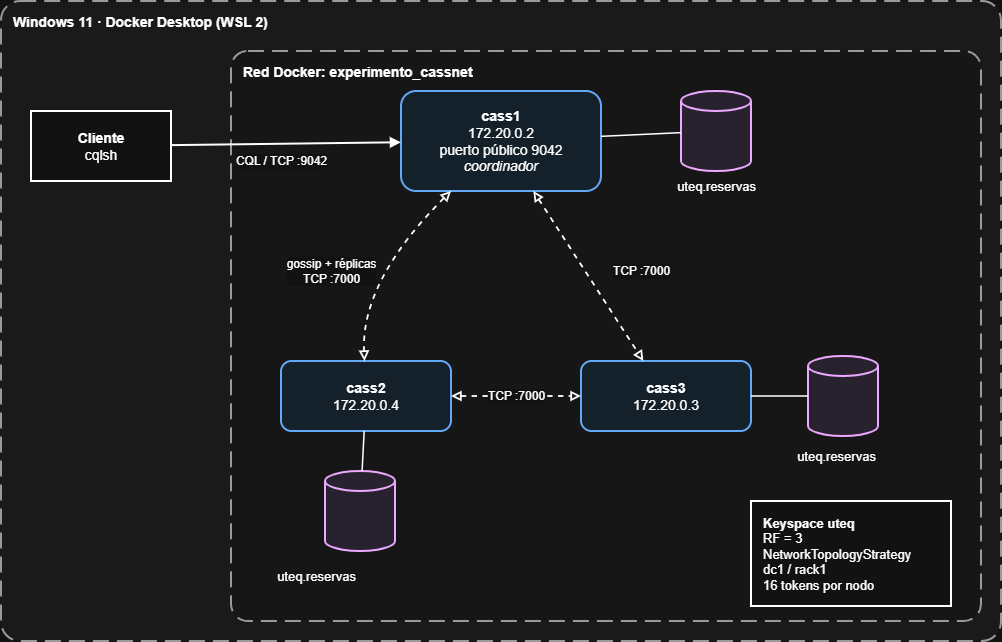
\includegraphics[width=0.9\textwidth]{Diagrama sin título.drawio.png}
  \caption{Arquitectura del clúster de Cassandra usado en el experimento (elaboración propia en draw.io a partir del esquema del Anexo A).}
  \label{fig:arquitectura}
\end{figure}

En el esquema a mano (Anexo A) no había anotado la IP de cass1 ni los puertos 7000 y 9042; los agregué en el diagrama de la Figura~\ref{fig:arquitectura} después de revisar los logs y \texttt{docker ps}.

% CUANDO TENGAS EL DIAGRAMA: sube figuras/arquitectura.png, descomenta la figura y agrega
% una o dos frases sobre qué cambiaste del esquema a mano (Anexo A) al diagrama de draw.io.
% \begin{figure}[H]
%   \centering
%   \includegraphics[width=0.9\textwidth]{figuras/arquitectura.png}
%   \caption{Arquitectura del clúster de Cassandra usado en el experimento (elaboración propia).}
%   \label{fig:arquitectura}
% \end{figure}

% ------------------------------------------------------------ 3
\section{Análisis con los conceptos de la Unidad 1}
\label{sec:analisis}

En esta sección reviso Cassandra con los conceptos de la Unidad 1: transparencias de distribución, CAP y PACELC, modelos de comunicación y tolerancia a fallos. En cada caso parto de lo que dicen las fuentes y lo contrasto con lo que observé en mi clúster de prueba, descrito en la Sección~\ref{sec:experimento}.

\subsection{Transparencias de distribución}

Una transparencia oculta al usuario algún aspecto de la distribución. La Tabla~\ref{tab:transparencias} resume cuáles ofrece Cassandra y qué vi de cada una en el experimento.

\begin{table}[H]
  \centering
  \caption{Transparencias de distribución en Cassandra.}
  \label{tab:transparencias}
  \begin{tabularx}{\textwidth}{llX}
    \toprule
    Transparencia & ¿La ofrece? & Lo que observé \\
    \midrule
    Acceso       & Sí      & Uso el mismo CQL sin importar a qué nodo me conecte. \\
    Ubicación    & Sí      & Consulté siempre por \texttt{cass1} sin saber en qué nodo estaba cada fila. \\
    Replicación  & Sí      & Hay tres copias de cada fila, pero la consulta devuelve una sola. \\
    Fallos       & Parcial & Con ONE y QUORUM no noté la caída de \texttt{cass3}; con ALL sí. \\
    Concurrencia & Parcial & No hay bloqueos; si dos clientes escriben la misma columna, gana la escritura más reciente. \\
    Migración y reubicación & Parcial & Al entrar un nodo se reparten los tokens sin cambiar nada en el cliente, pero el arranque necesitó intervención manual. \\
    \bottomrule
  \end{tabularx}
\end{table}

Las transparencias de acceso, ubicación y replicación son completas porque el coordinador hace todo el trabajo de buscar las réplicas. Las otras tres son parciales por decisión de diseño. La de fallos depende del nivel de consistencia que pida el cliente: con ALL el error llega hasta la aplicación. La de concurrencia funciona sin bloqueos, pero el precio es que una escritura puede sobrescribir otra sin aviso, porque Cassandra decide por la marca de tiempo. Y aunque agregar un nodo no cambia nada para el cliente, en mi caso tuve que arrancar \texttt{cass3} a mano porque dos nodos no pueden unirse al anillo al mismo tiempo.

\subsection{CAP y PACELC}

El teorema CAP plantea que, cuando hay una partición de red, un sistema distribuido debe elegir entre consistencia y disponibilidad. PACELC completa la idea: si no hay partición, la elección pasa a ser entre latencia y consistencia. Ahmed et al. clasifican a Cassandra como PA/EL, es decir, ante una partición prioriza la disponibilidad y en operación normal prioriza la baja latencia, y ubican a MongoDB como PA/EC \cite[p.~172]{ahmed2023consistency}.

Mi experimento coincide con esa clasificación, con un matiz. Apagar un nodo no es exactamente una partición, pero desde el coordinador se ve igual: hay una réplica que no contesta. En esa situación ONE y QUORUM siguieron respondiendo, que es el lado A, y ALL se negó, que es el lado C (Sección~\ref{sec:fallo}). Con los tres nodos arriba, pedir más consistencia costó más tiempo, de 1,2 ms con ONE a 5,2 ms con ALL, que es el intercambio entre L y C que describe PACELC. Por eso pienso que en Cassandra la posición en CAP no es fija para todo el sistema. La decide cada consulta según el nivel de consistencia que pide el cliente, y la etiqueta PA/EL describe lo que pasa con los niveles bajos, que son los que se usan por defecto.

\subsection{Modelos de comunicación}

Desde el punto de vista del cliente la comunicación es síncrona, porque \texttt{cqlsh} espera la respuesta antes de seguir. Dentro del clúster hay partes asíncronas. En una escritura con QUORUM, el coordinador envía el dato a las tres réplicas y contesta al cliente cuando dos confirman; la tercera termina de escribir después. Gossip también va por su lado: intercambia el estado de los nodos cada segundo, haya o no consultas.

\subsection{Tolerancia a fallos}

Con RF = 3 y operaciones en QUORUM, el clúster soporta la caída de un nodo sin dejar de responder y sin perder consistencia, porque siempre quedan dos réplicas que forman mayoría. Si caen dos nodos, solo ONE sigue funcionando.

Los fallos se detectan con gossip. Cada segundo los nodos intercambian su estado con otros nodos y, cuando uno deja de contestar, los demás lo marcan como caído. En mi prueba \texttt{cass3} apareció como DN en \texttt{nodetool status} casi en el momento en que lo detuve.

Para recuperarse, Cassandra tiene dos mecanismos. Con \textit{hinted handoff}, el coordinador guarda las escrituras que iban para el nodo caído y se las entrega cuando vuelve, siempre que no pasen más de tres horas (el valor por defecto). Con \textit{repair} (\texttt{nodetool repair}), los nodos comparan sus datos y copian a cada réplica lo que le falta, lo que cubre los casos en que esas pistas ya expiraron. En mi prueba no escribí datos mientras \texttt{cass3} estaba apagado, así que no llegué a ver el hinted handoff en acción.

Zhang et al. revisan los algoritmos de consenso tolerantes a fallos bizantinos, donde un nodo puede comportarse de forma arbitraria \cite{zhang2024byzantine}. Cassandra trabaja con un supuesto más simple: espera nodos que se caen, no nodos que mienten, y no usa consenso en cada escritura. Solo recurre a Paxos en las transacciones ligeras (\textit{lightweight transactions}).

% COMPLETA TU: si el caso de tu FORM-AC-01 es de una base distribuida, cuéntalo aquí
% en 3 o 4 frases (qué pasó, cuándo, qué falló y cómo se relaciona con gossip,
% réplicas o quórum).

% ------------------------------------------------------------ 4
\section{Experimentación propia}
\label{sec:experimento}

Las pruebas de esta sección las hice el 14 de noviembre de 2026 en mi computadora. Primero levanté el clúster, luego apagué un nodo para ver qué niveles de consistencia seguían respondiendo y, por último, con los tres nodos activos, medí cuánto tarda una lectura en cada nivel.

\subsection{Entorno}

Para comprobar lo que dicen las fuentes, levanté un clúster de Cassandra en mi propio equipo: una laptop con Windows 11, procesador Intel Core i7 de décima generación y 16 GB de RAM, con Docker Desktop sobre WSL 2. El clúster tiene tres nodos (\texttt{cass1}, \texttt{cass2} y \texttt{cass3}) con la imagen \texttt{cassandra:4.1}, todos en el centro de datos \texttt{dc1} y en \texttt{rack1}, conectados por una red de Docker llamada \texttt{experimento\_cassnet}. Creé el keyspace \texttt{uteq} con \texttt{NetworkTopologyStrategy} y factor de replicación 3, así que cada nodo guarda una copia completa de los datos. Dentro está la tabla \texttt{reservas} con dos filas de prueba. Solo \texttt{cass1} publica el puerto 9042 hacia mi máquina; los otros dos nodos se comunican únicamente dentro de la red de Docker. El \texttt{docker-compose.yml}, el script \texttt{experimento.cql}, los comandos y las salidas de cada prueba están en la carpeta \texttt{experimento/} del repositorio.

\subsection{Arranque y problema encontrado}

El primer intento no salió como esperaba. Ejecuté \texttt{docker compose up -d} a las 7:36 y, aunque los tres contenedores se crearon, a las 7:38 \texttt{nodetool status} mostraba un solo nodo en estado UN, el 172.20.0.2 (\texttt{cass1}). Medio minuto después apareció \texttt{cass2} en estado UJ (uniéndose) y, al revisar con \texttt{docker ps -a}, \texttt{cass3} había terminado con \texttt{Exited (3)}. Por lo que investigué, Cassandra no deja que dos nodos nuevos se unan al anillo al mismo tiempo: mientras uno está en estado \textit{Joining}, el otro debe esperar, y si intenta entrar igual se detiene. Lo resolví arrancando \texttt{cass3} a mano cuando \texttt{cass2} ya aparecía como UN. A las 7:44 los tres nodos ya estaban en UN, cada uno con 16 tokens. Esto me mostró que en un clúster real los nodos se agregan de uno en uno, aunque Docker Compose los levante todos con un solo comando.

\begin{figure}[H]
  \centering
  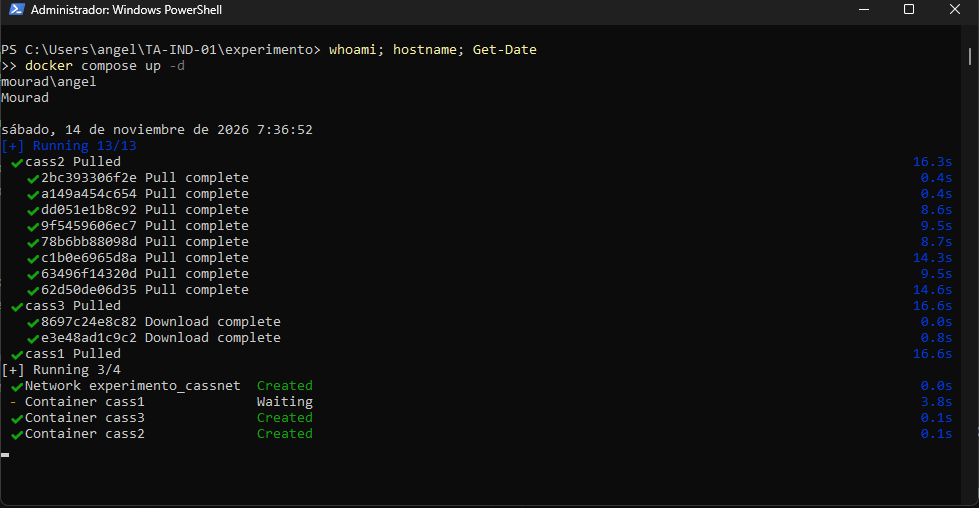
\includegraphics[width=0.85\textwidth]{Captura de pantalla 2026-11-14 073716.png}
  \caption{Arranque del clúster con \texttt{docker compose up -d} (14/11/2026, 7:36).}
\end{figure}

\begin{figure}[H]
  \centering
  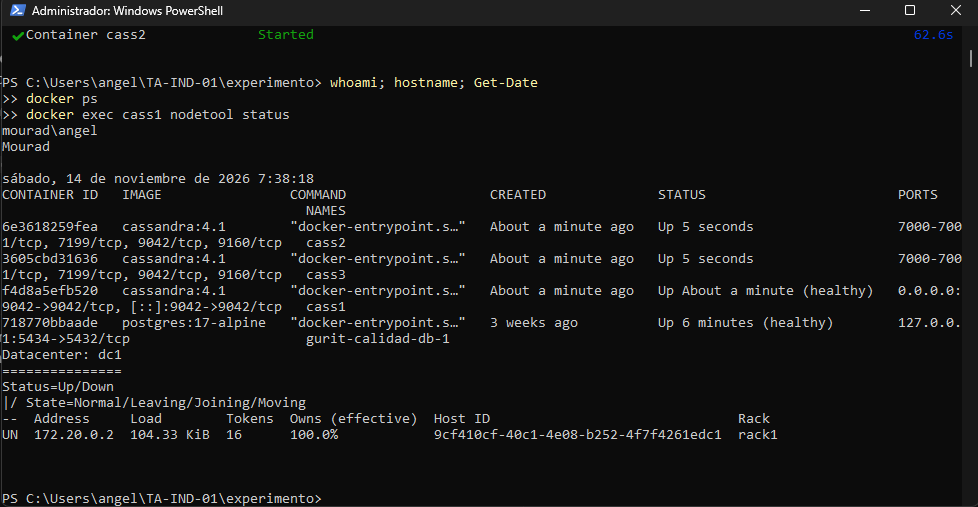
\includegraphics[width=0.85\textwidth]{Captura de pantalla 2026-11-14 073832.png}
  \caption{A las 7:38 solo \texttt{cass1} aparecía en estado UN.}
\end{figure}

\begin{figure}[H]
  \centering
  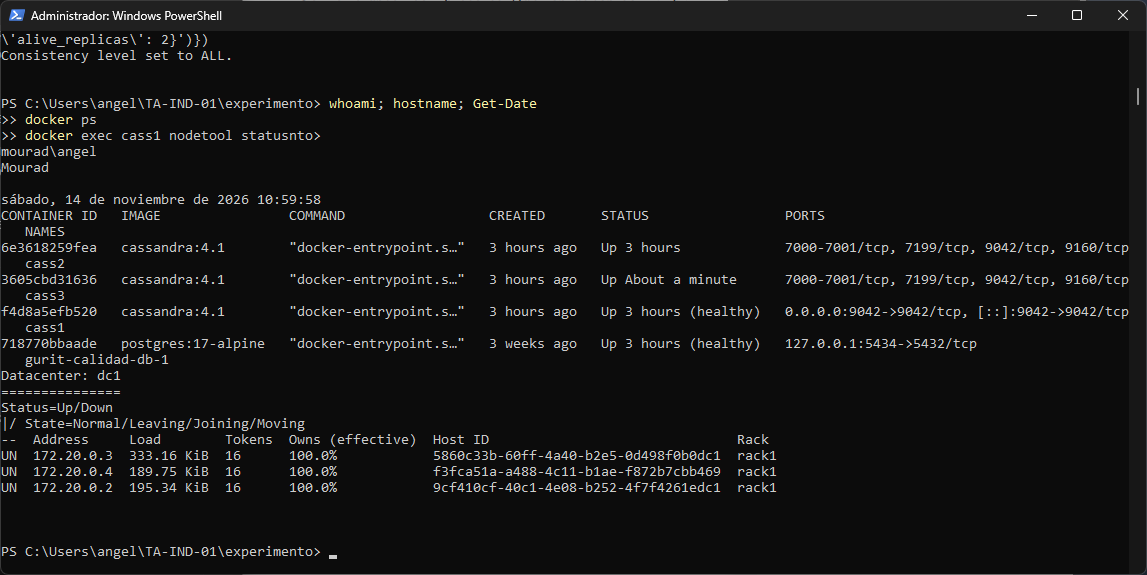
\includegraphics[width=0.85\textwidth]{Captura de pantalla 2026-11-14 110005.png}
  \caption{Los tres contenedores activos y los tres nodos en estado UN (repetición de la prueba, 10:59).}
\end{figure}

% \begin{figure}[H]
%   \centering
%   \includegraphics[width=0.85\textwidth]{Captura de pantalla 2026-11-14 XXXXXX.png}
%   \caption{Los tres nodos en estado UN según \texttt{nodetool status}.}
% \end{figure}

\subsection{Prueba de fallo de un nodo}
\label{sec:fallo}

Con el clúster completo cargué los datos con \texttt{experimento.cql} usando \texttt{CONSISTENCY ALL}, y la consulta devolvió las dos filas, señal de que las tres réplicas respondían. Luego detuve un nodo con \texttt{docker stop cass3} a las 7:45:40. \texttt{nodetool status} lo marcó como DN casi de inmediato, mientras \texttt{cass1} y \texttt{cass2} seguían en UN. Con el nodo caído leí la fila con \texttt{id = 1} desde \texttt{cass1} en los tres niveles de consistencia (Tabla~\ref{tab:fallo}). ONE y QUORUM devolvieron la fila sin problema. ALL falló a las 7:47:26 con el mensaje \textit{Cannot achieve consistency level ALL}, indicando \texttt{required\_replicas: 3} y \texttt{alive\_replicas: 2}. Las salidas completas quedaron guardadas en \texttt{one.txt}, \texttt{quorum.txt} y \texttt{all.txt}.

La explicación es aritmética simple. QUORUM pide la mayoría de las réplicas, 2 de 3, y con un nodo apagado todavía quedan dos copias vivas. ALL exige las tres y prefiere devolver un error antes que contestar con una réplica menos.

Para capturar la pantalla repetí la prueba entre las 10:58 y las 11:00 con el mismo resultado.

\begin{table}[H]
  \centering
  \caption{Lecturas con un nodo caído (2 de 3 réplicas vivas).}
  \label{tab:fallo}
  \begin{tabular}{lccl}
    \toprule
    Nivel & Réplicas necesarias & Vivas & Resultado \\
    \midrule
    ONE    & 1 & 2 & Devuelve la fila \\
    QUORUM & 2 & 2 & Devuelve la fila \\
    ALL    & 3 & 2 & Error (no disponible) \\
    \bottomrule
  \end{tabular}
\end{table}

\begin{figure}[H]
  \centering
  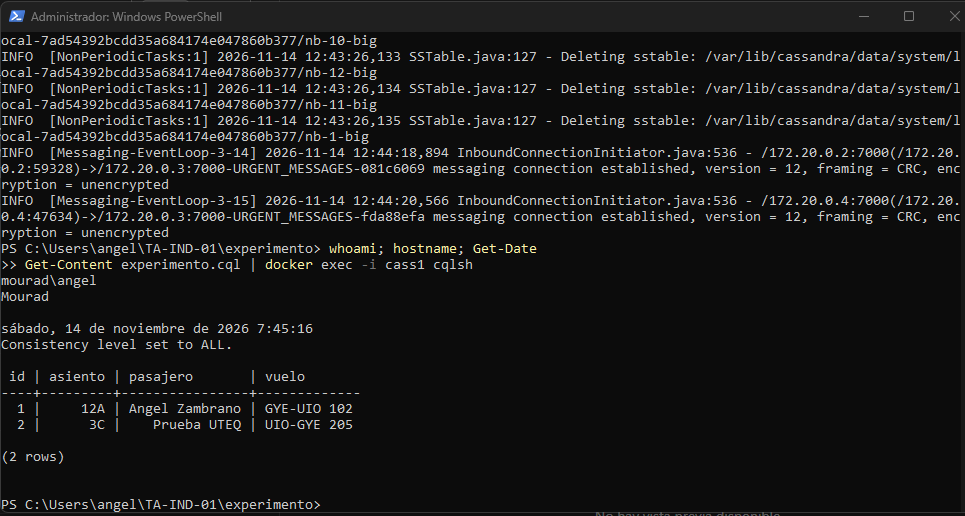
\includegraphics[width=0.85\textwidth]{Captura de pantalla 2026-11-14 074527.png}
  \caption{Datos cargados con \texttt{CONSISTENCY ALL} antes de la prueba de fallo (7:45).}
\end{figure}

\begin{figure}[H]
  \centering
  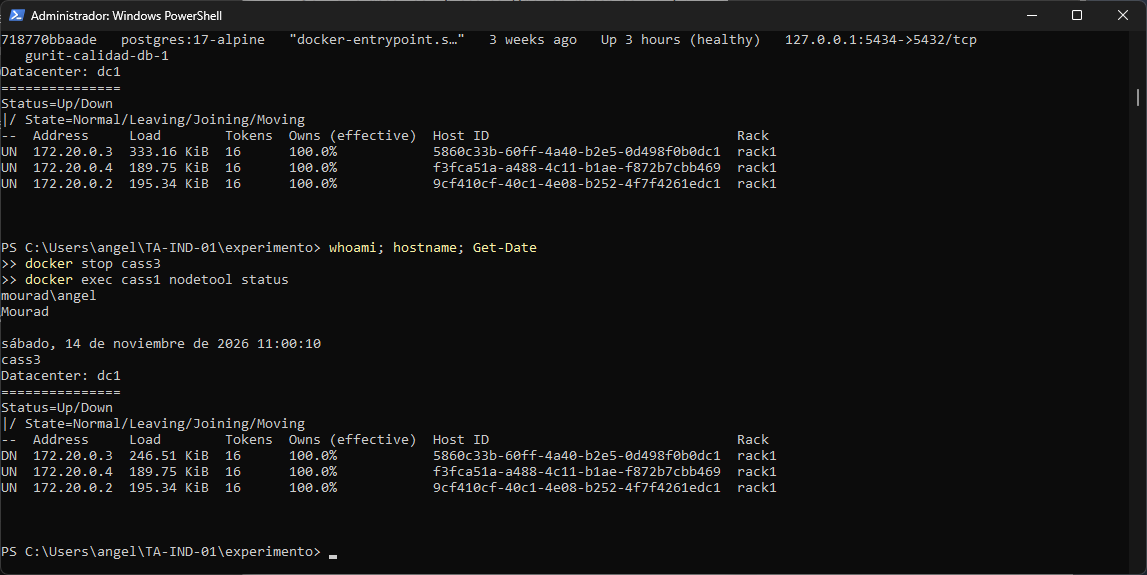
\includegraphics[width=0.85\textwidth]{Captura de pantalla 2026-11-14 110016.png}
  \caption{\texttt{cass3} detenido y marcado como DN; \texttt{cass1} y \texttt{cass2} siguen en UN (11:00).}
\end{figure}

\begin{figure}[H]
  \centering
  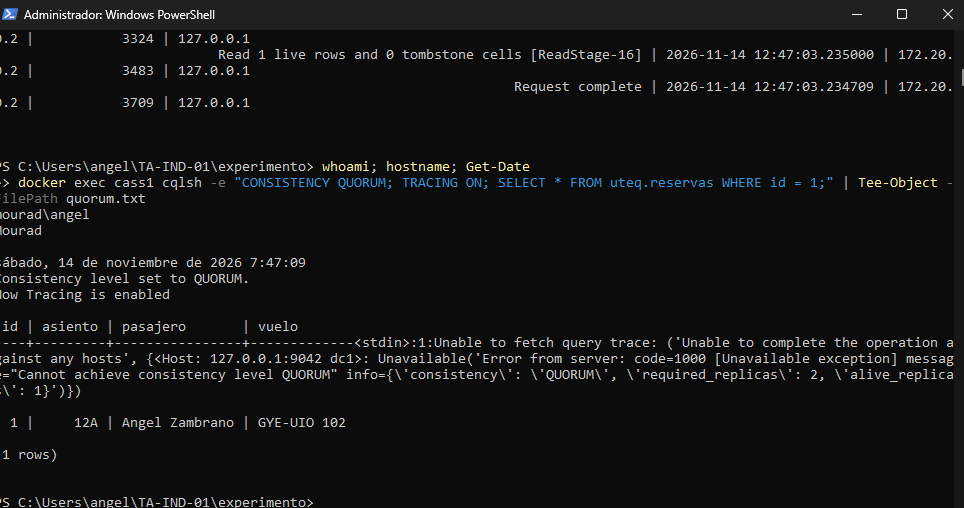
\includegraphics[width=0.85\textwidth]{Captura de pantalla 2026-11-14 074720.png}
  \caption{Lectura con QUORUM con un nodo caído (7:47): la fila se devuelve, pero falla la lectura de la traza en \texttt{system\_traces}.}
\end{figure}

\begin{figure}[H]
  \centering
  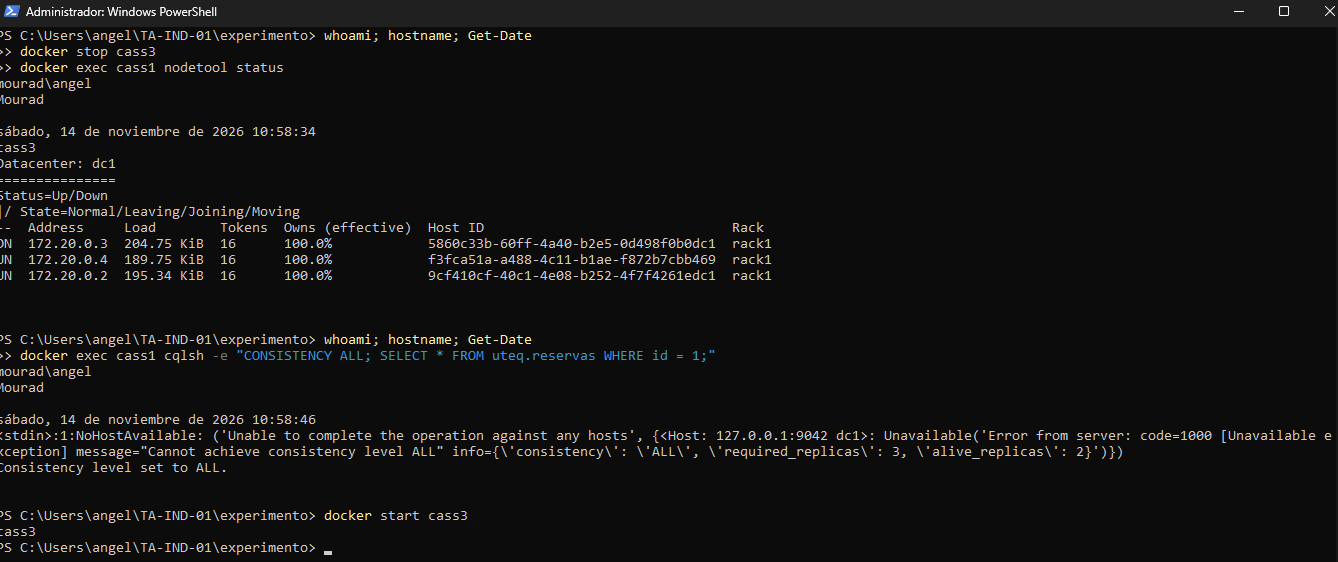
\includegraphics[width=0.85\textwidth]{Captura de pantalla 2026-11-14 105857.png}
  \caption{Lectura con ALL rechazada con un nodo caído: \texttt{required\_replicas: 3}, \texttt{alive\_replicas: 2} (10:58).}
\end{figure}

Hubo un detalle que no esperaba. Al activar \texttt{TRACING ON} con QUORUM, la fila sí llegó, pero \texttt{cqlsh} mostró \textit{Unable to fetch query trace} con \texttt{required\_replicas: 2} y \texttt{alive\_replicas: 1}. El error no venía de \texttt{uteq} sino de \texttt{system\_traces}, el keyspace donde Cassandra guarda las trazas, que por defecto tiene factor de replicación 2. Con \texttt{cass3} apagado, una de las dos copias de esa traza no estaba disponible, y QUORUM sobre RF = 2 necesita ambas. Así entendí que el factor de replicación se define por keyspace y que dos keyspaces del mismo clúster pueden reaccionar distinto ante la misma falla.



% \begin{figure}[H]
%   \centering
%   \includegraphics[width=0.85\textwidth]{Captura de pantalla 2026-11-14 XXXXXX.png}
%   \caption{\texttt{cass3} detenido y marcado como DN.}
% \end{figure}


% \begin{figure}[H]
%   \centering
%   \includegraphics[width=0.85\textwidth]{Captura de pantalla 2026-11-14 XXXXXX.png}
%   \caption{Lectura con ALL rechazada: \texttt{required\_replicas: 3}, \texttt{alive\_replicas: 2}.}
% \end{figure}



\subsection{Latencia según el nivel de consistencia}

Con los tres nodos activos otra vez, medí cuánto tarda la misma lectura (la fila \texttt{id = 1}, consultada desde \texttt{cass1}) con cada nivel. Usé un bucle en PowerShell de cinco rondas que en cada una ejecuta la consulta con ONE, QUORUM y ALL y toma el tiempo de la línea \textit{Request complete} del tracing. Los 15 valores quedaron en \texttt{latencias.txt} y el resumen está en la Tabla~\ref{tab:latencia}.

\begin{table}[H]
  \centering
  \caption{Latencia de lectura con los 3 nodos activos, 5 rondas (µs).}
  \label{tab:latencia}
  \begin{tabular}{lrrrr}
    \toprule
    Nivel & Promedio & Mínimo & Máximo & Desv. est. \\
    \midrule
    ONE    & 1237,8 & 1141 & 1333 &  77,5 \\
    QUORUM & 3822,8 & 3448 & 4255 & 319,6 \\
    ALL    & 5212,6 & 4163 & 6111 & 846,8 \\
    \bottomrule
  \end{tabular}
\end{table}

\begin{figure}[H]
  \centering
  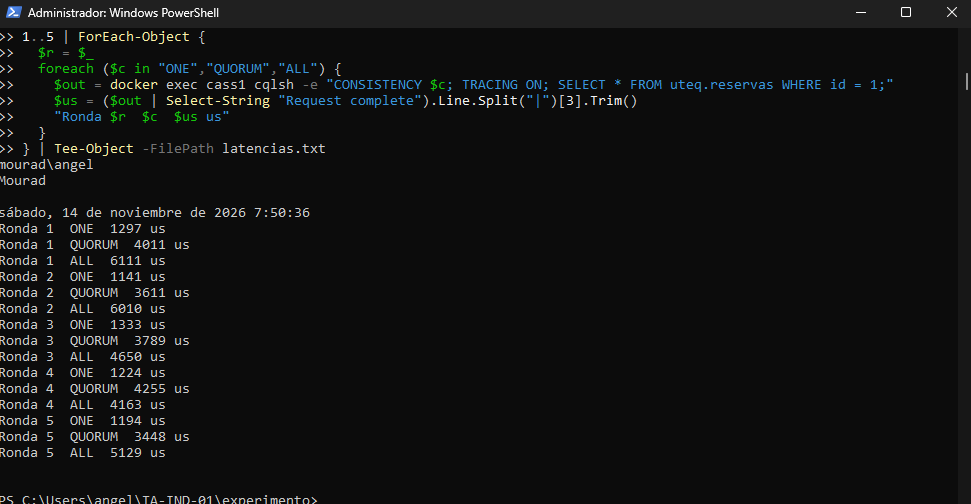
\includegraphics[width=0.85\textwidth]{Captura de pantalla 2026-11-14 075131.png}
  \caption{Quince mediciones de latencia guardadas en \texttt{latencias.txt} (7:50).}
\end{figure}

En promedio QUORUM tardó unas 3 veces lo que ONE y ALL unas 4 veces. El orden ONE, QUORUM, ALL se cumplió en cuatro de las cinco rondas. En la ronda 4, ALL marcó 4163\,\textmu s y quedó por debajo de QUORUM, que marcó 4255\,\textmu s. Creo que pasó porque los tres nodos corren en la misma máquina y comparten CPU y disco con Docker y con el resto de Windows, así que cualquier proceso en segundo plano puede retrasar una medición suelta. ALL fue además el nivel que más varió (desviación de 846,8\,\textmu s frente a 77,5 de ONE). Tiene sentido: el coordinador espera a la réplica más lenta de las tres, y cuál es la más lenta cambia de una ronda a otra.

La prueba tiene límites claros. Todo corre en un solo equipo, sin distancia de red entre los nodos, y son apenas cinco rondas. Gorbenko et al. encontraron diferencias de hasta 600\,\% entre niveles de consistencia con réplicas en regiones distintas \cite{gorbenko2021performance}. En mi caso la diferencia viene casi solo del trabajo de coordinar réplicas, porque los mensajes entre contenedores no salen de la máquina.


% Capturas: pon las imágenes en figuras/ y descomenta.
% \begin{figure}[H]
%   \centering
%   \includegraphics[width=0.9\textwidth]{figuras/07_all_falla.png}
%   \caption{Lectura con ALL rechazada con un nodo caído.}
% \end{figure}

% ------------------------------------------------------------ 5
\section{Ejemplos de mi entorno}
% REVISA: el ingeniero pide solo cosas que de verdad te pasaron. Cambia cualquier
% detalle que no sea exacto (fechas, qué viste en pantalla).

El primer ejemplo es el SGA de la UTEQ. En las semanas de matrículas y en las noches antes de que cierre una entrega, la plataforma se pone lenta y a veces una página no termina de cargar o me saca de la sesión. Muchos estudiantes entran al mismo tiempo y el servidor no alcanza a atender todas las peticiones. Esto tiene que ver con la disponibilidad y la escalabilidad: un sistema que funciona bien con carga normal deja de responder cuando la carga se multiplica. Cassandra ataca ese problema agregando nodos, porque cualquiera de ellos puede atender consultas.

El segundo ejemplo es WhatsApp. Me ha pasado que envío un mensaje y se queda con un solo visto porque la otra persona no tiene conexión; cuando vuelve a conectarse, el mensaje le llega y aparecen los dos vistos. Es comunicación asíncrona: el mensaje queda guardado en el servidor y se entrega cuando el destinatario está disponible, sin que yo tenga que esperar con la aplicación abierta. Se parece al \textit{hinted handoff} de Cassandra, donde el coordinador guarda las escrituras para un nodo caído y se las entrega cuando vuelve.

% ------------------------------------------------------------ 6
\section{Análisis comparativo}

\begin{table}[H]
  \centering
  \caption{Comparación de Apache Cassandra y MongoDB.}
  \label{tab:comparacion}
  \begin{tabularx}{\textwidth}{lXX}
    \toprule
    Criterio & Apache Cassandra & MongoDB \\
    \midrule
    Arquitectura & Sin maestro; anillo de nodos iguales. & Conjunto de réplicas con un nodo primario y varios secundarios. \\
    CAP / PACELC & PA/EL \cite[p.~172]{ahmed2023consistency}. & PA/EC \cite[p.~172]{ahmed2023consistency}. \\
    Replicación & Multimaestro; cualquier réplica acepta escrituras y el RF se define por keyspace. & Las escrituras van al primario y los secundarios copian su registro de operaciones. \\
    Comunicación & Peer-to-peer entre nodos y CQL entre cliente y coordinador. & El cliente escribe en el primario; los secundarios replican desde él. \\
    Tolerancia a fallos & Sigue respondiendo según el nivel de consistencia pedido. & Si cae el primario, los secundarios eligen uno nuevo y mientras tanto no se aceptan escrituras. \\
    \bottomrule
  \end{tabularx}
\end{table}

La diferencia de fondo está en quién puede escribir. En Cassandra cualquier nodo acepta escrituras, así que la carga se reparte y la caída de un nodo no detiene al sistema. En MongoDB todas las escrituras pasan por el primario, lo que hace más fácil leer siempre el dato más reciente, pero cuando el primario cae hay unos segundos sin escrituras hasta que se elige uno nuevo.

Por eso, para una aplicación con muchas escrituras repartidas, como registros de sensores, historiales de actividad o mensajes, Cassandra encaja mejor. Para una aplicación donde importa leer siempre el valor actualizado y el volumen de escrituras es moderado, MongoDB es más sencillo de usar sin pensar en niveles de consistencia. Ferreira et al. estudian justamente cómo cambian el rendimiento y el comportamiento de estas bases según el nivel de consistencia configurado \cite{ferreira2024impacts,ferreira2025experimental}, y mi experimento muestra la misma idea a escala pequeña: en Cassandra la consistencia fuerte existe, pero hay que pedirla y pagarla en latencia.
% REVISA: si en tus PDFs de Ferreira hay un número concreto (por ejemplo, cuánto baja el
% rendimiento con QUORUM o ALL), agrégalo aquí con la página.
\newpage
% ------------------------------------------------------------ 7
\section{Postura crítica}

La mayor fortaleza de Cassandra es que sigue funcionando con nodos caídos. En mi prueba, con un nodo apagado, dos de los tres niveles de consistencia respondieron sin problema. A eso se suma que para crecer basta con agregar nodos, sin un servidor principal que se vuelva cuello de botella.

Sus limitaciones también salieron en el experimento. La consistencia fuerte es cara: leer con ALL tomó unas 4 veces más que con ONE, y eso que los nodos estaban en la misma máquina. El modelado de datos es rígido, porque las tablas se diseñan según las consultas que se van a hacer y no hay \texttt{JOIN}; si mañana cambia la consulta, muchas veces hay que crear otra tabla. La operación tampoco es simple: solo levantar tres nodos me dio el problema del arranque simultáneo, y en producción hay que programar \texttt{repair}, vigilar el gossip y planificar cómo entra cada nodo.

No usaría Cassandra para un sistema contable o de inventario de un negocio pequeño, por ejemplo una tienda con unos pocos miles de productos. Ahí cada venta toca varias tablas a la vez (factura, detalle, stock, caja) y todo tiene que quedar consistente en el mismo instante. Una base relacional como PostgreSQL resuelve eso con transacciones en un solo servidor, que alcanza de sobra para ese volumen. Con Cassandra tendría que repartir esa lógica en la aplicación y pagar la complejidad de un clúster que no necesito.

% ------------------------------------------------------------ 8
\section{Conclusiones}

En mi clúster de tres nodos, leer con ALL tomó en promedio 5,2 ms frente a 1,2 ms con ONE y 3,8 ms con QUORUM, así que cada nivel más fuerte se paga en latencia aunque no haya red de por medio. Con un nodo caído, ONE y QUORUM siguieron devolviendo la fila y ALL falló con \texttt{alive\_replicas: 2}, lo que confirma la clasificación PA/EL de Ahmed et al.\ siempre que el cliente use niveles bajos. El error de tracing sobre \texttt{system\_traces} me mostró que el factor de replicación es una decisión por keyspace y que conviene revisarlo también en los keyspaces del sistema. Por último, el fallo al arrancar los tres nodos a la vez dejó claro que la tolerancia a fallos de Cassandra no elimina el trabajo de operarla con cuidado.

% ------------------------------------------------------------ 9
\section*{Declaración de uso de inteligencia artificial}

Usé Claude (Anthropic), modelo Claude Opus 5.5, para preparar el \texttt{docker-compose.yml} y los comandos del experimento; ordenar en \texttt{resultados.txt} y \texttt{comandos.md} las salidas que obtuve en mi terminal; armar la estructura del archivo \LaTeX{} y del archivo de referencias; proponer un guion con las preguntas de cada sección; redactar la Introducción y los párrafos de apertura de las Secciones 3 y 4 a partir de mis textos, y revisar la redacción y las horas del experimento contra mi registro de PowerShell. Las demás secciones las redacté yo. Para verificar, ejecuté todos los comandos en mi equipo, comparé cada número del informe con mis capturas y con los archivos de \texttt{experimento/}, y abrí cada DOI para comprobar autores, año, título, revista, volumen y páginas.
\newpage
% ------------------------------------------------------------ REFERENCIAS
\printbibliography[title={Referencias}]
\newpage
% ------------------------------------------------------------ ANEXOS
\appendix
\section{Esquema inicial a mano}

Este es el primer esquema del clúster que dibujé a mano antes de montar el experimento, con mi nombre y la fecha.
% Sube la foto a figuras/esquema_a_mano.jpg y descomenta.
\begin{figure}[H]
\centering
 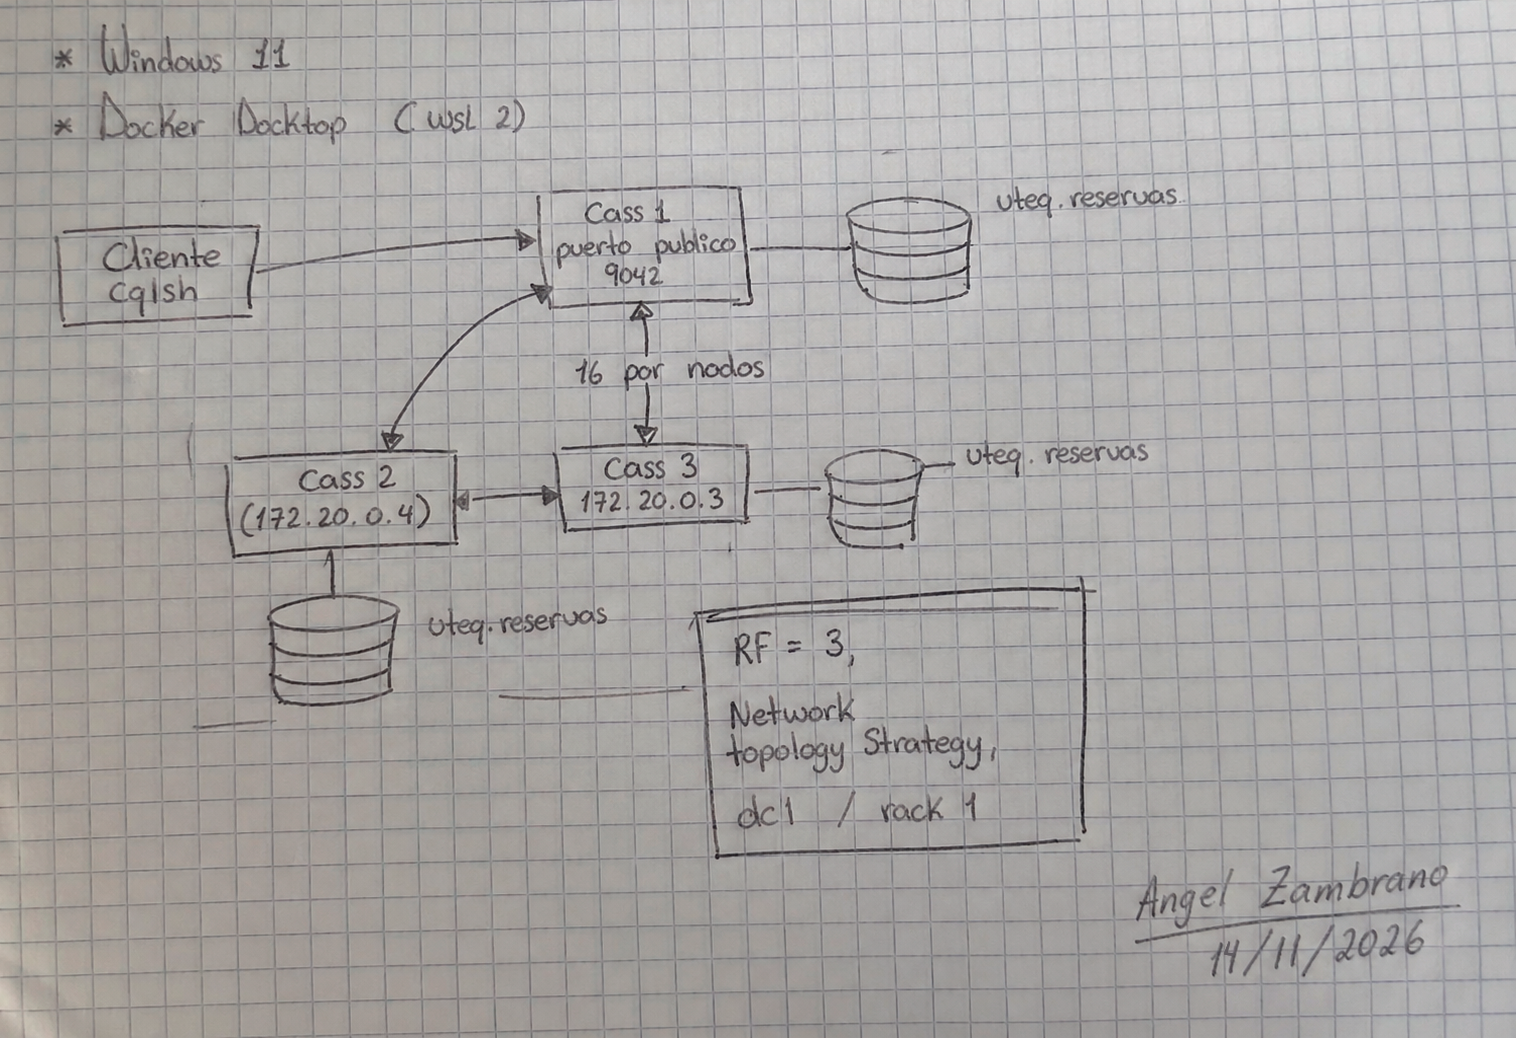
\includegraphics[width=0.8\textwidth]{Diagrama-Cassandra-en-cuaderno-cuadriculado.png}
 \caption{Esquema inicial a mano.}
 \label{fig:esquema}
 \end{figure}


 
\newpage
\section{Capturas de lectura de las fuentes}
Estas capturas muestran los pasajes que resalté en los artículos y que cito en el informe.



\begin{figure}[H]
  \centering
  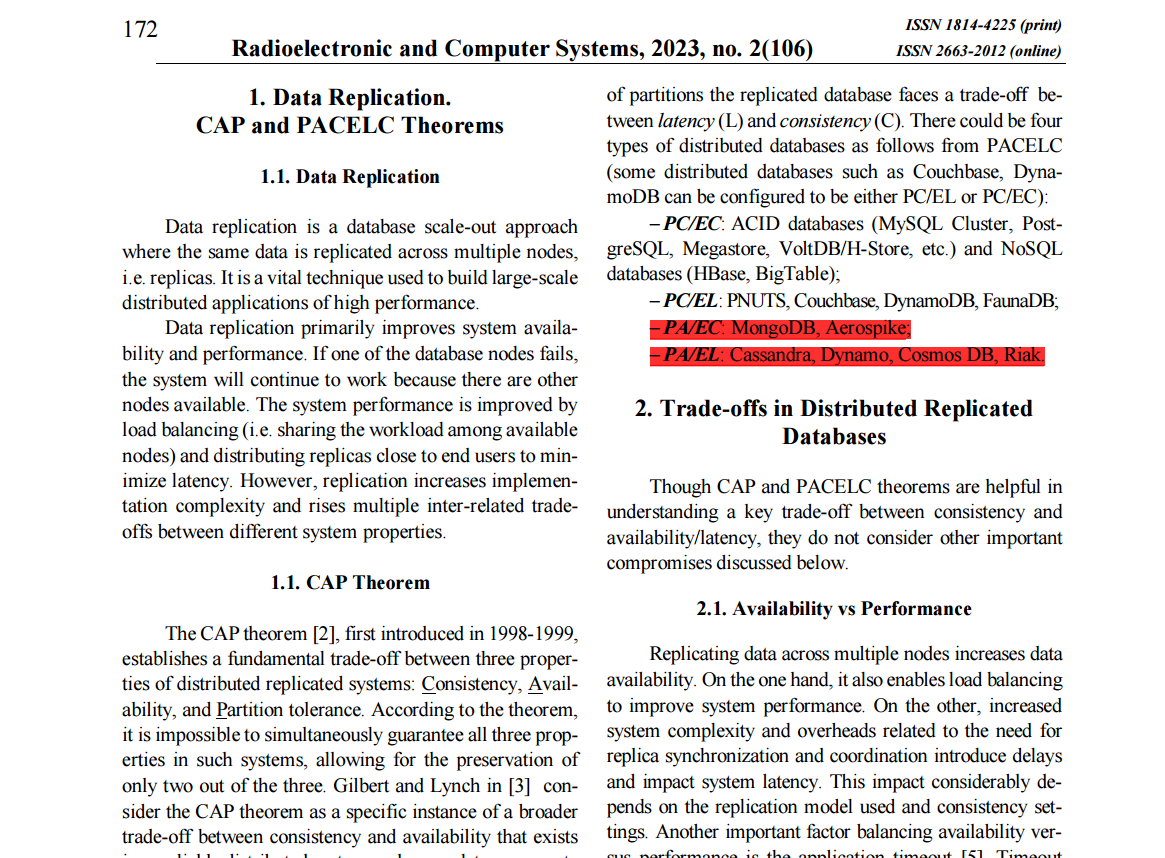
\includegraphics[width=0.7\textwidth]{lectura_ahmed_p172.png}
  \caption{Ahmed et al., p.~172: clasificación PACELC de Cassandra (PA/EL) y MongoDB (PA/EC). Citado en la Sección~3.2 y en la Tabla~4 \cite[p.~172]{ahmed2023consistency}.}
\end{figure}

\begin{figure}[H]
  \centering
  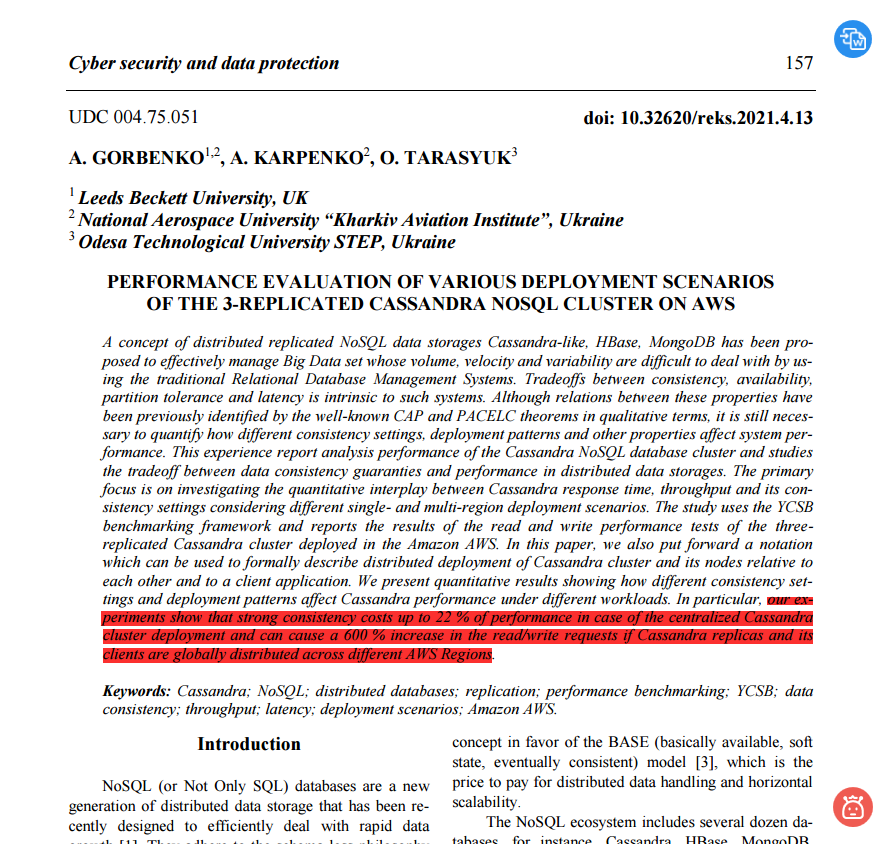
\includegraphics[width=0.7\textwidth]{lectura_gorbenko_p157.png}
  \caption{Gorbenko et al., p.~157: costo de la consistencia fuerte (hasta 22\,\% centralizado y 600\,\% entre regiones). Citado en la Sección~4.4 \cite{gorbenko2021performance}.}
\end{figure}

\begin{figure}[H]
  \centering
  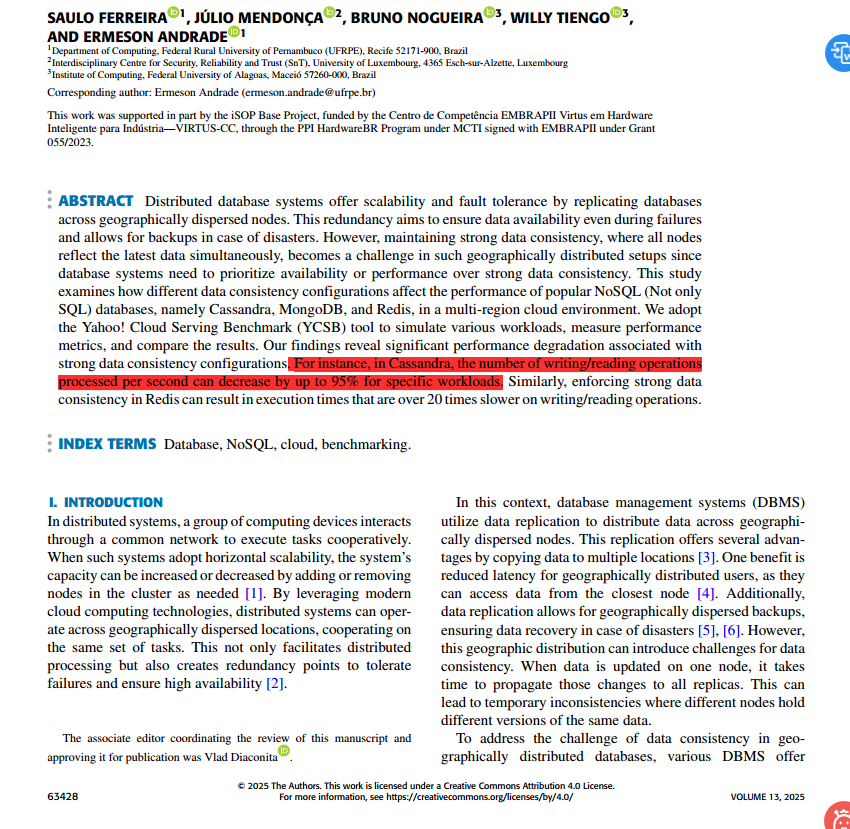
\includegraphics[width=0.7\textwidth]{lectura_ferreira_p63428.png}
  \caption{Ferreira et al., p.~63428: caída de hasta 95\,\% en las operaciones por segundo de Cassandra con consistencia fuerte. Citado en la Introducción \cite{ferreira2025benchmarking}.}
\end{figure}

\end{document}
